\documentclass[aspectratio=1610]{beamer}
\usetheme{metropolis}
\titlegraphic{
    
\includegraphics[height=0.13\textheight]{./img/oxlogo.eps}
  \hfill
  
\includegraphics[height=0.13\textheight]{./img/InFoMM.eps}
}

\title{Shape Optimization Using Nearly Conformal Mappings}
\date{October 31, 2017 - JAMS}
\author{Florian Wechsung, Kevin Sturm, Jos\'e A. Iglesias}
\usepackage{mathtools}
\mathtoolsset{showonlyrefs}
%\usepackage{graphics}
%\usepackage{amsmath}

\usepackage{changepage}
\usepackage{animate}
\usepackage[noplaybutton]{media9}
\usepackage[colorlinks]{hyperref}
\usepackage{attachfile2}
\usefonttheme[onlymath]{serif}
\usepackage{wasysym}
\usepackage{xparse}
%\usepackage[firstpage]{draftwatermark} %http://choorucode.com/2010/05/05/latex-adding-draft-watermark/
%\usepackage{eulervm}
%\renewcommand{\rmdefault}{pplx}
% \usepackage{perpage} %the perpage package
% \MakePerPage{footnote} %the perpage package command
% \usepackage{mathtools}
% \mathtoolsset{showonlyrefs=true,showmanualtags=true}
\newcommand{\re}{\mathbb{R}}
\newcommand{\com}{\mathbb{C}}
\newcommand{\nat}{\mathbb{N}}
\newcommand{\rat}{\mathbb{Q}}

\newcommand{\Rey}{\mathrm{Re}}
\newcommand{\sym}{\mathrm{sym}}

\newcommand{\tet}{\vartheta}
\newcommand{\Tet}{\Theta}

\newcommand{\eps}{\varepsilon}
\renewcommand{\l}{\left}
\renewcommand{\r}{\right}
\let\temp\phi
\let\phi\varphi
\let\varphi\temp
\renewcommand{\div}{\mathrm{\div}}

\newcommand{\Ra}{\Rightarrow}
\newcommand{\ra}{\rightarrow}

\newcommand{\pkt}{\boldsymbol{\cdot}}
\def\longrightharpoonup{\relbar\joinrel\rightharpoonup}
\newcommand{\Ac}{\mathcal{A}}
\newcommand{\Bc}{\mathcal{B}}
\newcommand{\Cc}{\mathcal{C}}
\newcommand{\Dc}{\mathcal{D}}
\newcommand{\Ec}{\mathcal{E}}
\newcommand{\Fc}{\mathcal{F}}
\newcommand{\Gc}{\mathcal{G}}
\newcommand{\Hc}{\mathcal{H}}
\newcommand{\Jc}{\mathcal{J}}
\newcommand{\Kc}{\mathcal{K}}
\newcommand{\Lc}{\mathcal{L}}
\newcommand{\Mc}{\mathcal{M}}
\newcommand{\Nc}{\mathcal{N}}
\newcommand{\Oc}{\mathcal{O}}
\newcommand{\Pc}{\mathcal{P}}
\newcommand{\Qc}{\mathcal{Q}}
\newcommand{\Rc}{\mathcal{R}}
\newcommand{\Sc}{\mathcal{S}}
\newcommand{\Tc}{\mathcal{T}}
\newcommand{\Uc}{\mathcal{U}}
\newcommand{\Vc}{\mathcal{V}}
\newcommand{\Wc}{\mathcal{W}}
\newcommand{\Xc}{\mathcal{X}}
\newcommand{\Yc}{\mathcal{Y}}

\newcommand{\idb}{\mathbf{id}}
\newcommand{\fb}{\mathbf{f}}
\newcommand{\nb}{\mathbf{n}}
\renewcommand{\sb}{\mathbf{s}}
\newcommand{\ub}{\mathbf{u}}
\newcommand{\vb}{\mathbf{v}}
\newcommand{\xb}{\mathbf{x}}
\newcommand{\zb}{\mathbf{z}}

\newcommand{\Cb}{\mathbb{C}}
\newcommand{\Eb}{\mathbb{E}}
\newcommand{\Hb}{\mathbb{H}}
\newcommand{\Ib}{\mathbf{I}}
\newcommand{\Pb}{\mathbb{P}}
\newcommand{\Qb}{\mathbb{Q}}
\newcommand{\Kb}{\mathbb{K}}
\newcommand{\Nb}{\mathbb{N}}
\newcommand{\Ub}{\mathbb{U}}
\newcommand{\Vb}{\mathbb{V}\mathrm{ar}}
\newcommand{\Zb}{\mathbb{Z}}

\newcommand{\bbf}{\mathbf{b}}
\newcommand{\Id}{\mathrm{Id}}
\newcommand{\Lip}{\mathrm{Lip}}
\newcommand{\lLip}{\underline{\mathrm{Lip}}}

\def\Proj_#1{\ensuremath{\operatorname{Proj}_{#1}\!}}
\newcommand{\ind}{\mathbf{1}}
\newcommand{\ilquote}[1]{``#1''}
\newcommand{\dr}[1]{\ensuremath{\operatorname{d}\!{#1}}}
\newcommand{\Dr}[1]{\ensuremath{\operatorname{D}\!{#1}}}
\def\Drs_#1{\ensuremath{\operatorname{D}_{#1}\!}}
\def\Drs^#1{\ensuremath{\operatorname{D}^{#1}\!}}
\newcommand{\Er}[1]{\ensuremath{\operatorname{E}\!{#1}}}
\def\Ers_#1{\mathrm{E}_{#1}}
\newcommand{\dm}{\mathrm{dim}}
\newcommand{\Cov}{\mathrm{Cov}}
\newcommand{\Corr}{\mathrm{Corr}}

\newcommand{\aufz}{\leavevmode\vspace{-\baselineskip}}

\DeclareMathOperator{\dist}{dist}
\DeclareMathOperator*{\esup}{ess\,sup}
\DeclareMathOperator*{\argmin}{arg\,min}
\DeclareMathOperator*{\argmax}{arg\,max}
\DeclareMathOperator{\diam}{diam}
\newcommand{\const}{\mathrm{const}}
\DeclareMathOperator{\tr}{{tr}}
\DeclareMathOperator{\Tr}{{Tr}}
\DeclareMathOperator{\supp}{supp}
\let\div\relax
\DeclareMathOperator{\div}{div}
\DeclareMathOperator{\curl}{curl}
\newcommand{\uX}{\underline{X}}
\newcommand{\ux}{\underline{x}}
\newcommand{\mres}{\mathbin{\vrule height 1.6ex depth 0pt width
0.13ex\vrule height 0.13ex depth 0pt width 1.3ex}}
\newcommand{\defeq}{\vcentcolon=}
\newcommand{\eqdef}{=\vcentcolon}
\newcommand{\loc}{\mathrm{loc}}

\def\xunderbrace#1_#2{{\underbrace{#1}_{\mathclap{#2}}}}
\def\xoverbrace#1^#2{{\overbrace{#1}^{\mathclap{#2}}}}
\def\xunderarrow#1_#2{{\underset{\overset{\uparrow}{\mathclap{#2}}}{#1}}}
\def\xoverarrow#1^#2{{\overset{\underset{\downarrow}{\mathclap{#2}}}{#1}}}
\let\weakto\rightharpoonup
\providecommand{\abs}[1]{\left\lvert#1\right\rvert}
\providecommand{\norm}[1]{\left\lVert#1\right\rVert}
\providecommand{\set}[1]{\left\{#1\right\}}
\newcommand{\trenner}[2]{
    \begin{flushright}[#1]%
        \vspace{0.001mm}%
        \hrule %
        \vspace{-0.02mm}%
[#2]\end{flushright}}

\DeclareDocumentCommand{\boxedeq}{m o}{%
    \IfNoValueTF{#2}{%
        \rlap{\boxed{#1}}%
        \phantom{\hskip\fboxrule\hskip\fboxsep #1}%
        }{%
        \rlap{\boxed{#1#2}}%
        \phantom{\hskip\fboxrule\hskip\fboxsep #1}&\phantom{#2}%
    }%
}



\newcommand{\E}[2]{
    \mathbb{E}_{#1}\l[#2\r]
}
\renewcommand{\P}[1]{
    \mathbb{P}\l(#1\r)
}
\renewcommand{\=}[2]{
    \overset{\mathsmaller{#1}}{\underset{\mathsmaller{#2}}=}
}
\catcode`@=11

\def\nvphantom{\v@true\h@false\nph@nt}
\def\nhphantom{\v@false\h@true\nph@nt}
\def\nphantom{\v@true\h@true\nph@nt}
\def\nph@nt{\ifmmode\def\next{\mathpalette\nmathph@nt}%
\else\let\next\nmakeph@nt\fi\next}
\def\nmakeph@nt#1{\setbox\z@\hbox{#1}\nfinph@nt}
\def\nmathph@nt#1#2{\setbox\z@\hbox{$\m@th#1{#2}$}\nfinph@nt}
\def\nfinph@nt{\setbox\tw@\null
    \ifv@ \ht\tw@\ht\z@ \dp\tw@\dp\z@\fi
\ifh@ \wd\tw@-\wd\z@\fi \box\tw@}

\def\Xint#1{\mathchoice
    {\XXint\displaystyle\textstyle{#1}}%
    {\XXint\textstyle\scriptstyle{#1}}%
    {\XXint\scriptstyle\scriptscriptstyle{#1}}%
    {\XXint\scriptscriptstyle\scriptscriptstyle{#1}}%
\!\int}
\def\XXint#1#2#3{{\setbox0=\hbox{$#1{#2#3}{\int}$ }
\vcenter{\hbox{$#2#3$ }}\kern-.6\wd0}}
\def\ddashint{\Xint=}
\def\dashint{\Xint-}

\newcommand{\claim}[1]{\textbf{Claim:} #1\\}
\newcommand{\step}[2]{\textbf{Step #1:} #2\\}
\newcommand{\subproof}{\textit{Proof: }}
\newcommand{\phantomsign}{\hphantom{{ }+{ }}}
\newcommand{\myplus}{{{ }+{ }}}
\newcommand{\myminus}{{{ }-{ }}}


\usepackage{tikz}
\usepackage{pgfplots}
\pgfdeclarelayer{background}% determine background layer
\pgfsetlayers{background,main}% order of layers
\tikzset{
    invisible/.style={opacity=0},
    visible on/.style={alt={#1{}{invisible}}},
    alt/.code args={<#1>#2#3}{%
      \alt<#1>{\pgfkeysalso{#2}}{\pgfkeysalso{#3}} % \pgfkeysalso doesn't change the path
    },
  }
\definecolor{seaborn1}{rgb}{0.2980392156862745, 0.4470588235294118, 0.6901960784313725}
\definecolor{seaborn2}{rgb}{0.3333333333333333, 0.6588235294117647, 0.40784313725490196}
\definecolor{seaborn3}{rgb}{0.7686274509803922, 0.3058823529411765, 0.3215686274509804}
\definecolor{seaborn4}{rgb}{0.5058823529411764, 0.4470588235294118, 0.6980392156862745}
\definecolor{seaborn5}{rgb}{0.8, 0.7254901960784313, 0.4549019607843137}
\definecolor{seaborn6}{rgb}{0.39215686274509803, 0.7098039215686275, 0.803921568627451}
\definecolor{blue}{rgb}{0.2980392156862745, 0.4470588235294118, 0.6901960784313725}
\definecolor{green}{rgb}{0.3333333333333333, 0.6588235294117647, 0.40784313725490196}
\definecolor{red}{rgb}{0.7686274509803922, 0.3058823529411765, 0.3215686274509804}
\newenvironment{variableblock}[3]{%
  \setbeamercolor{block body}{#2}
  \setbeamercolor{block title}{#3}
  \begin{block}{#1}}{\end{block}}

\newenvironment{challengeblock}[1]{%
  \begin{variableblock}{#1}{bg=seaborn3!20,fg=black}{bg=seaborn3,fg=white}}{\end{variableblock}}
\renewenvironment{exampleblock}[1]{%
  \begin{variableblock}{#1}{bg=green!20,fg=black}{bg=green,fg=white}}{\end{variableblock}}
\newenvironment{answerblock}[1]{%
  \begin{variableblock}{#1}{bg=blue!20,fg=black}{bg=blue,fg=white}}{\end{variableblock}}
\newenvironment{ideablock}[1]{%
  \begin{variableblock}{#1}{bg=seaborn5!20,fg=black}{bg=seaborn5,fg=white}}{\end{variableblock}}
\usepackage{microtype}
\newcommand{\CR}{\mathrm{CR}}

\newcommand{\includemovie}[2][]{
    \includemedia[
        #1,
        activate=pageopen,transparent,
        addresource=#2.mp4,addresource=#2.png,
        flashvars={
            file=#2.mp4&image=#2.png&
            stretching=uniform&start=0&
            screencolor=white& %improves render in light backgrounds
            controlbar.position=over&controlbar.idlehide=true&
            autostart=true&repeat=always&smoothing=true
            %&bufferlength=10 % may improve repetition of short videos
        }
    ]{ % for disabled content (in most cases this is fallback)
        \begin{tabular}{ll}
            \mbox{
            %   \href{run:#2.mp4} % for not embedded fallback
                \textattachfile[color={0 0 0}]{#2.mp4} % for embedded fallback
                {
                \texttt{|\kern-.23em>}
                } % poor play button
            } & \raisebox{-\height}{\includegraphics[#1]{#2}}
        \end{tabular}
    }{player.swf}
}
\begin{document}
\maketitle
%\begin{frame}[t]{Overview}
%    \tableofcontents
%\end{frame}
\begin{frame}[t]{Shape Optimization}
    \begin{challengeblock}{Challenge}
        Find a shape that minimizes a functional subject to constraints.
    \end{challengeblock}

    \only<2->{
        \begin{equation}
            \begin{aligned}
                & \underset{\Omega}{\text{minimize}}
                & & J(\Omega, u)\\
                &\text{ subject to } && \Omega \in K\\
                &&& e_{\Omega}(u) = 0
            \end{aligned}
        \end{equation}
    }
    \only<3->{
        \vfill
        \begin{minipage}{0.49\textwidth}
            Functionals:
            \begin{itemize}
                \item Drag / lift, 
                \item Energy dissipation,
                \item Compliance
                    \item $\dots$
            \end{itemize}
        \end{minipage}
        \begin{minipage}{0.49\textwidth}
            Constraints:
            \begin{itemize}
                \item Volume
                \item Barycentre
                \item Minimum lift
                    \item \dots
            \end{itemize}
        \end{minipage}
    }
\end{frame}
\begin{frame}[t]{Example}
    Maximize the aerodynamic efficiency of an airfoil subject to a box constraint.   \vfill
    \begin{figure}
        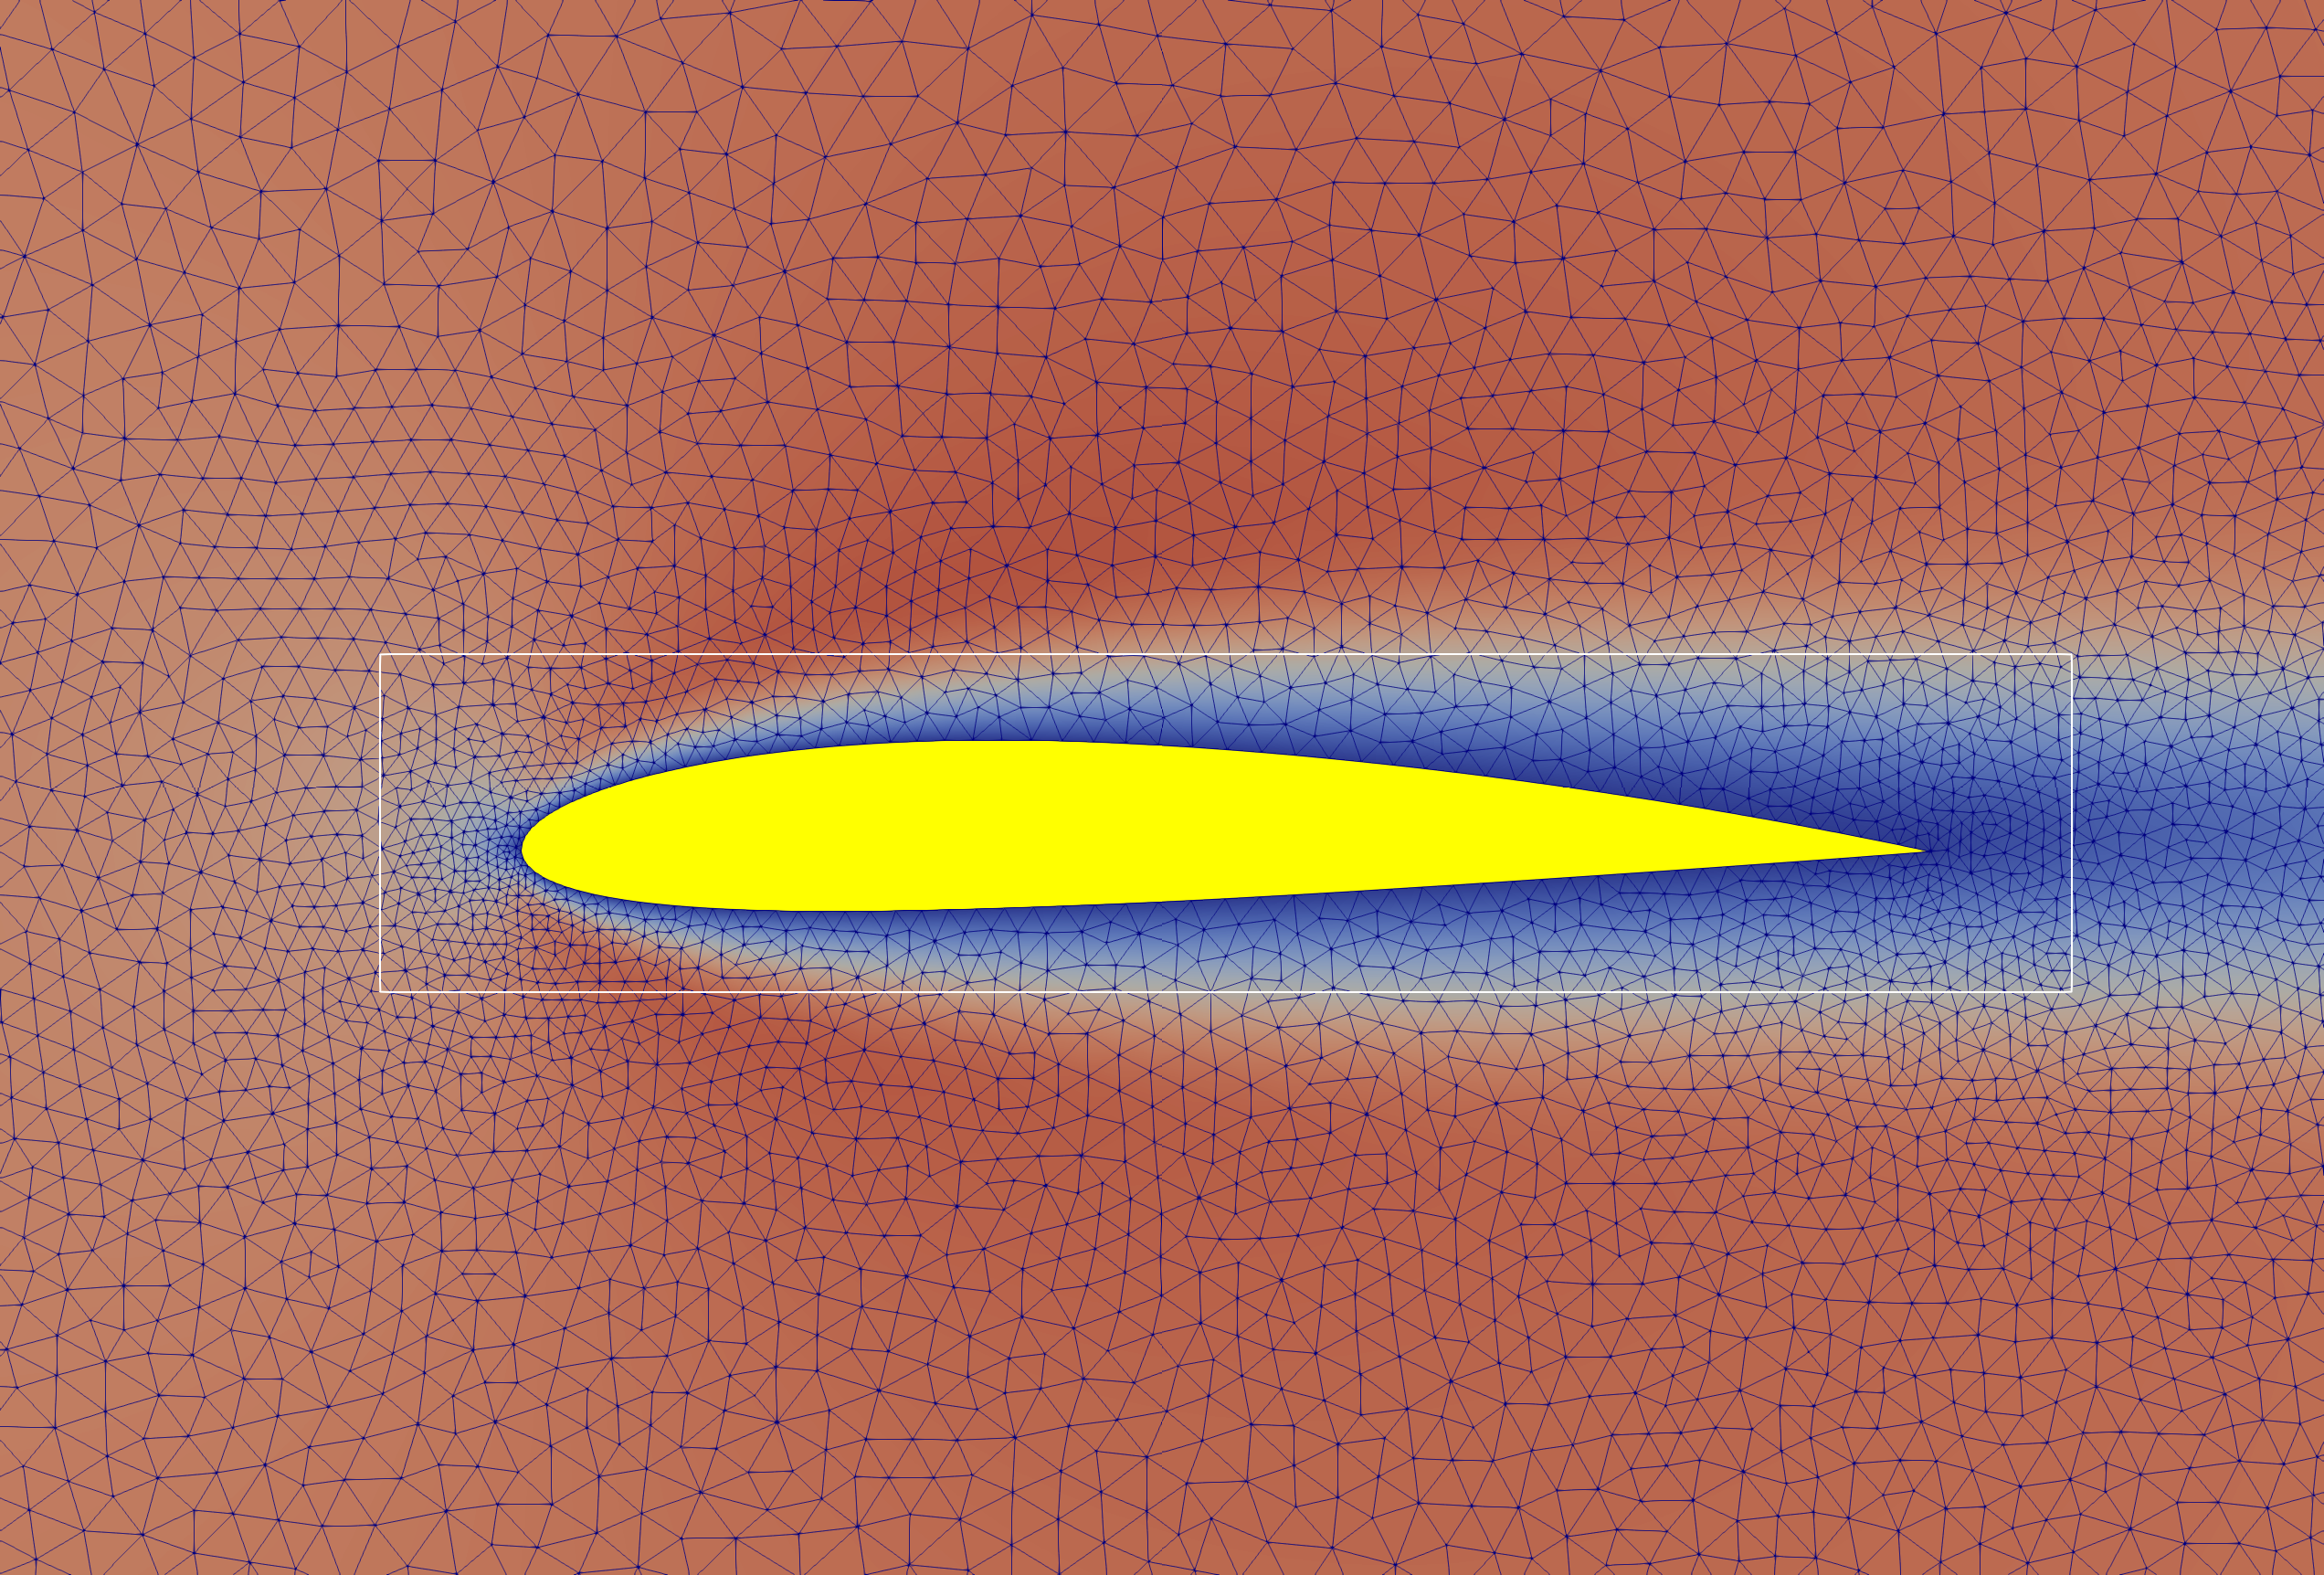
\includegraphics[width=0.48\linewidth]{./img/airfoil_init.png} \hfill
        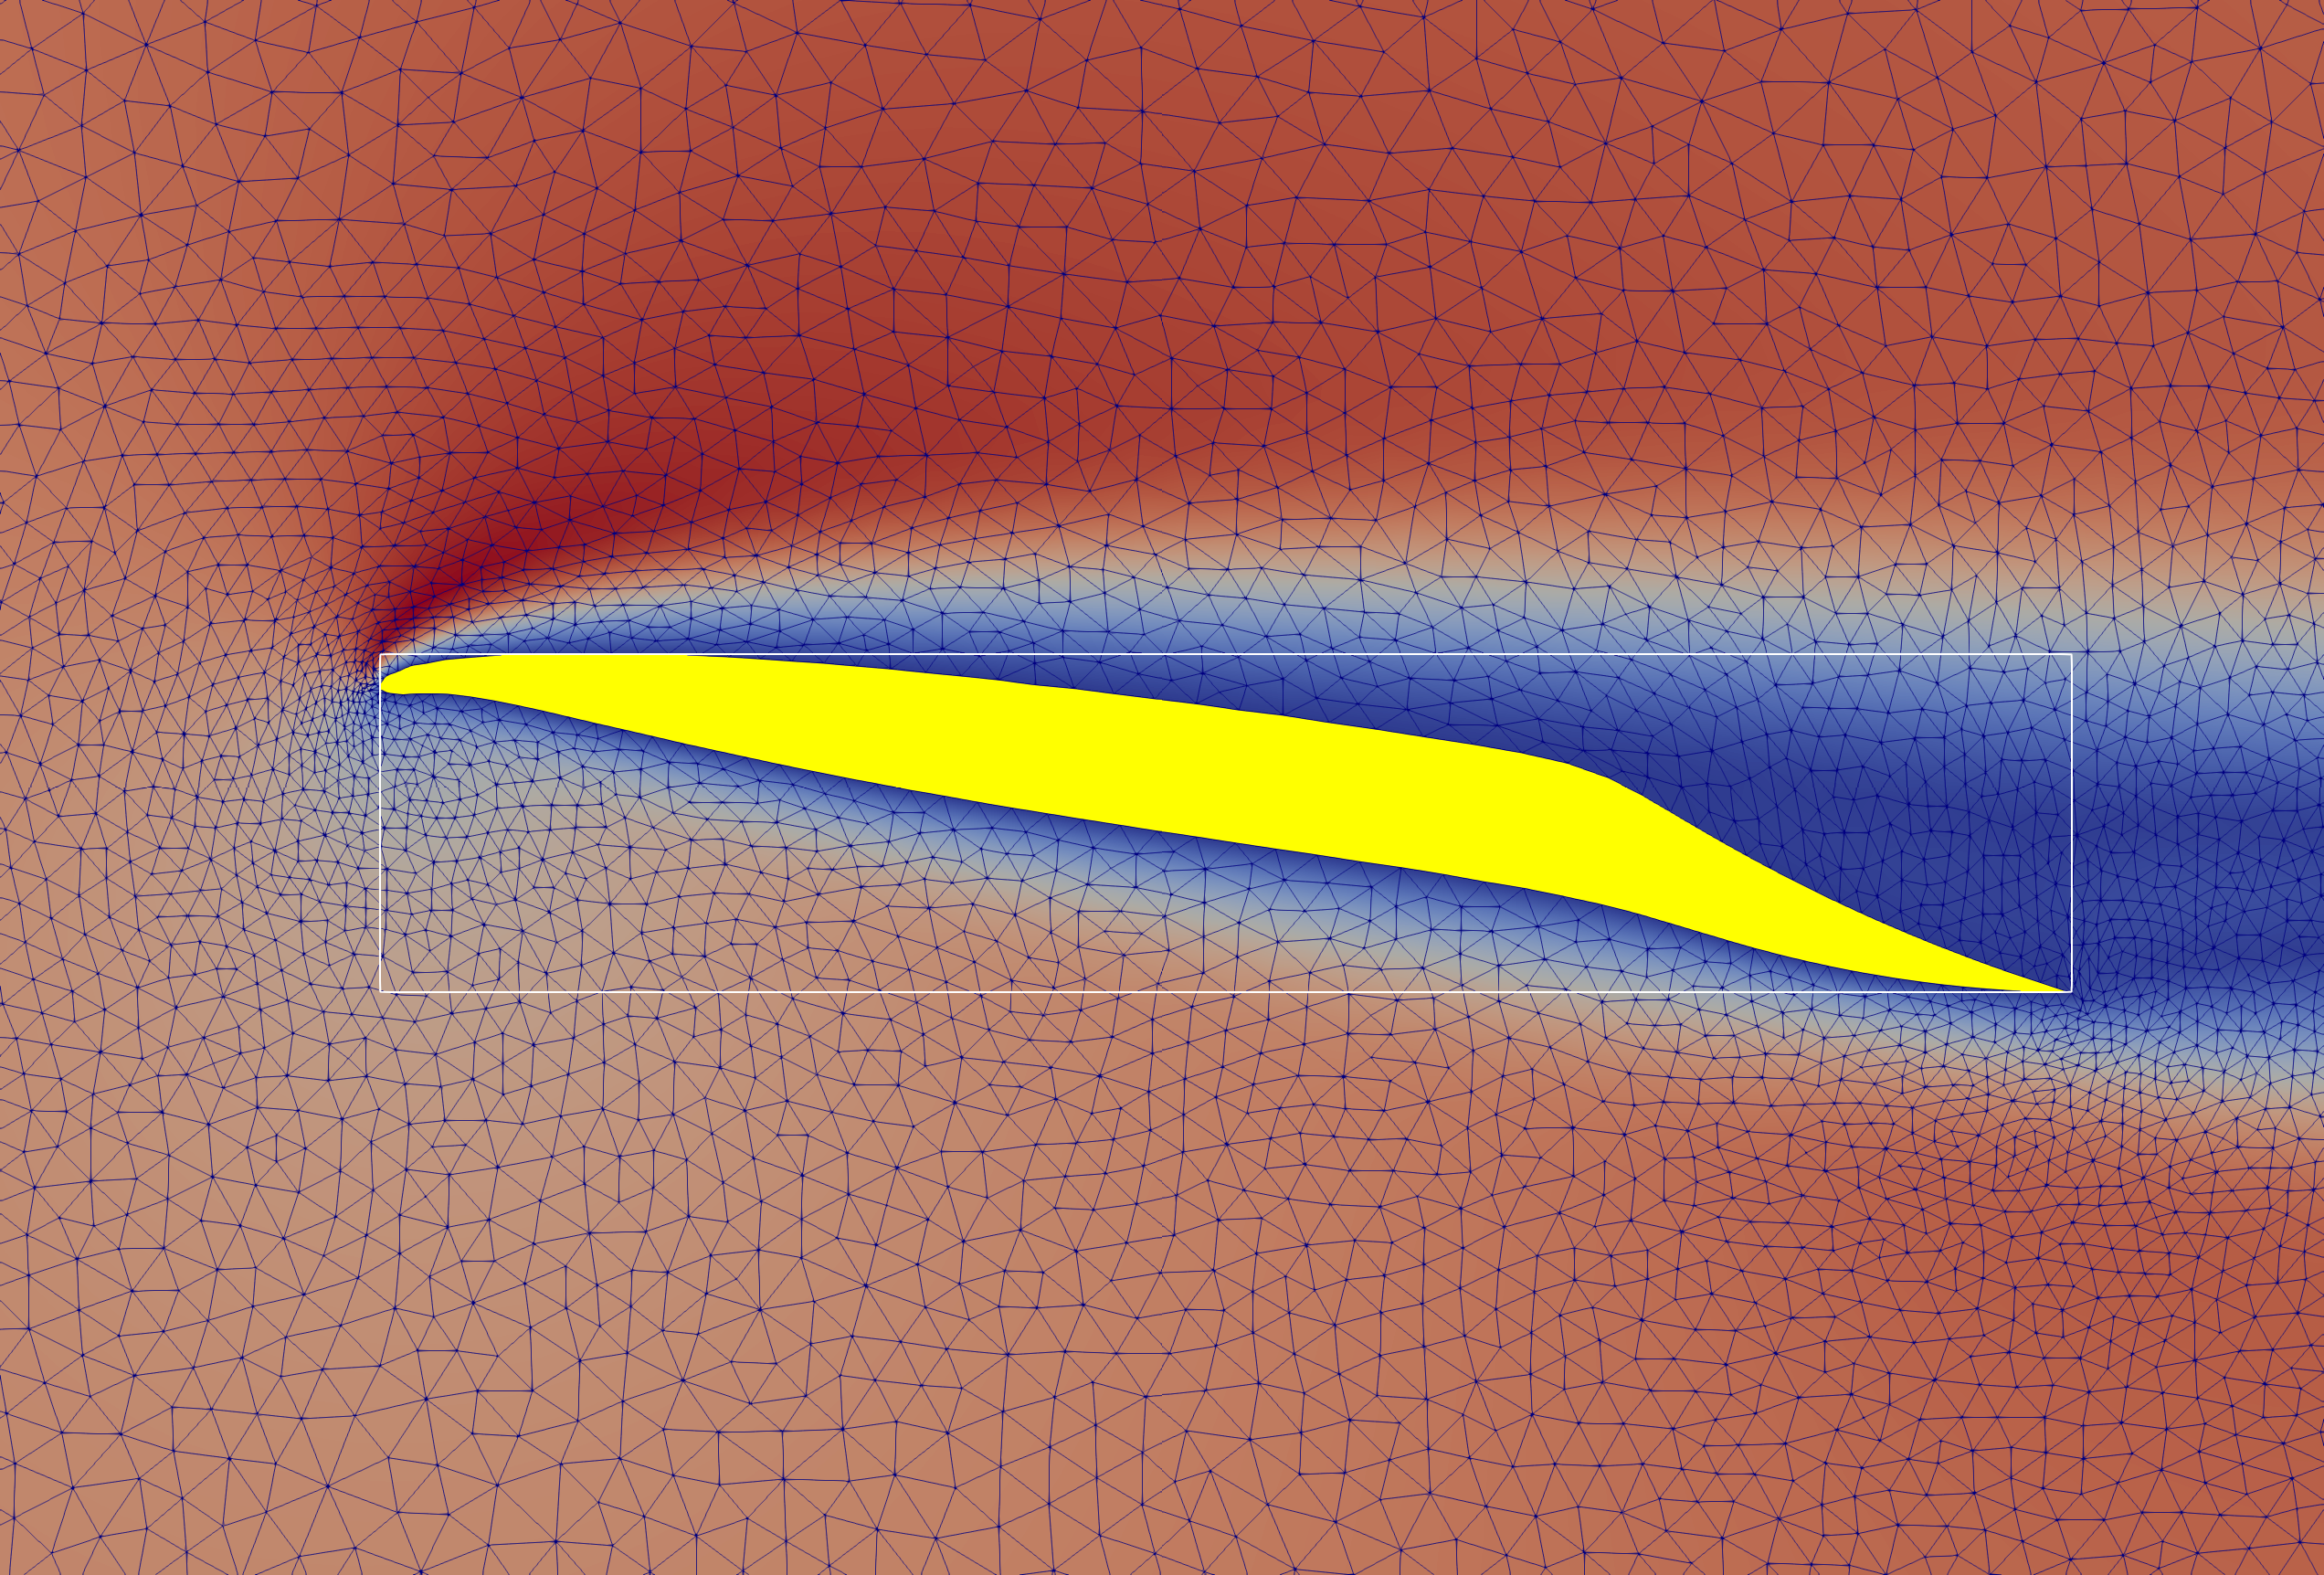
\includegraphics[width=0.48\linewidth]{./img/airfoil_final.png}
        \caption{Initial shape and optimized shape}
    \end{figure}
    \vspace{-0.5cm}
    \begin{itemize}
        \item PDE constraint: Navier-Stokes equations.
        \item Geometric constraint: constant volume \& box constraint.
    \end{itemize}
\end{frame}
\begin{frame}
        %\includemedia[
        %width=1\linewidth,
        %keepaspectratio,
        %addresource=./img/airfoil.mp4,
        %flashvars={source=./img/airfoil.mp4}
        %]{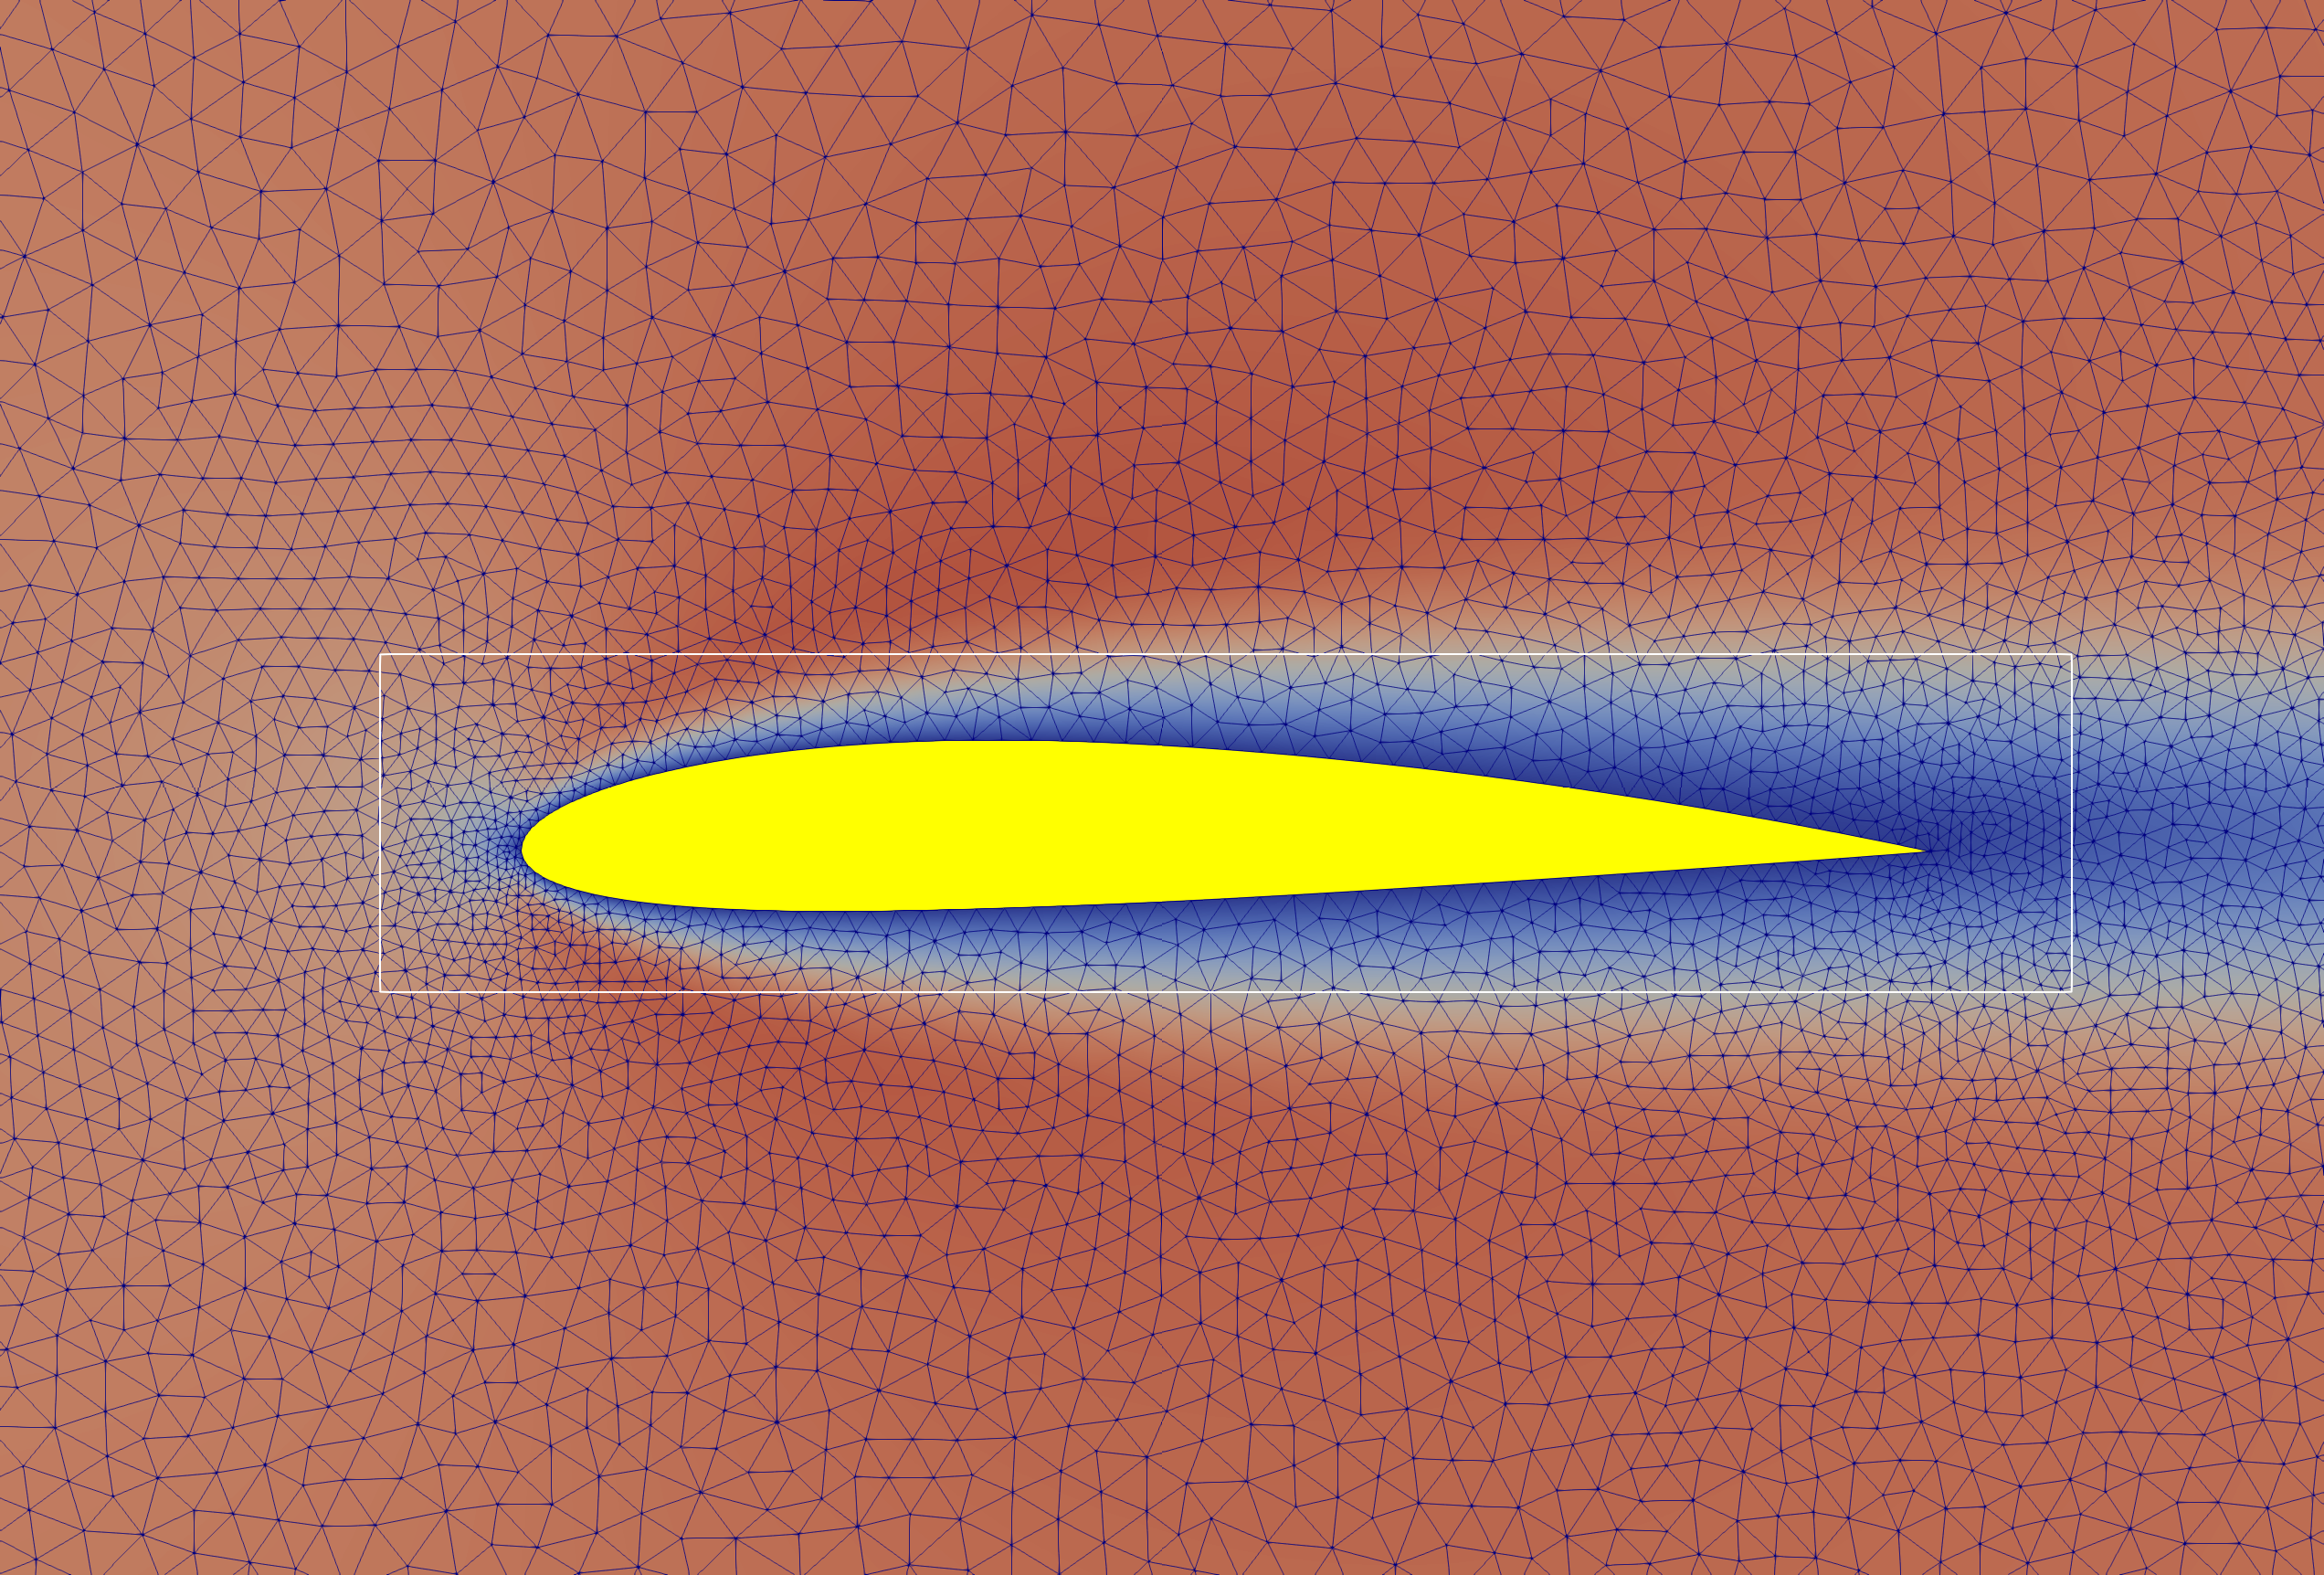
\includegraphics[width=\linewidth]{./img/airfoil_init.png}}{VPlayer.swf}
    \includemovie[width=\textwidth]{img/airfoil}
\end{frame}
\begin{frame}{Mesh deformation}
    When we deform the mesh we need to ensure that
    \begin{itemize}
        \item elements to not start overlapping;
        \item elements do not become overly stretched.
    \end{itemize}
    \begin{challengeblock}{Problem}
        We need to find ways of deforming the finite element mesh without reducing its quality.
    \end{challengeblock}
\end{frame}
\begin{frame}{Example}
    Consider the toy problem of mapping a circle to a clover-like shape:
    \begin{center}
        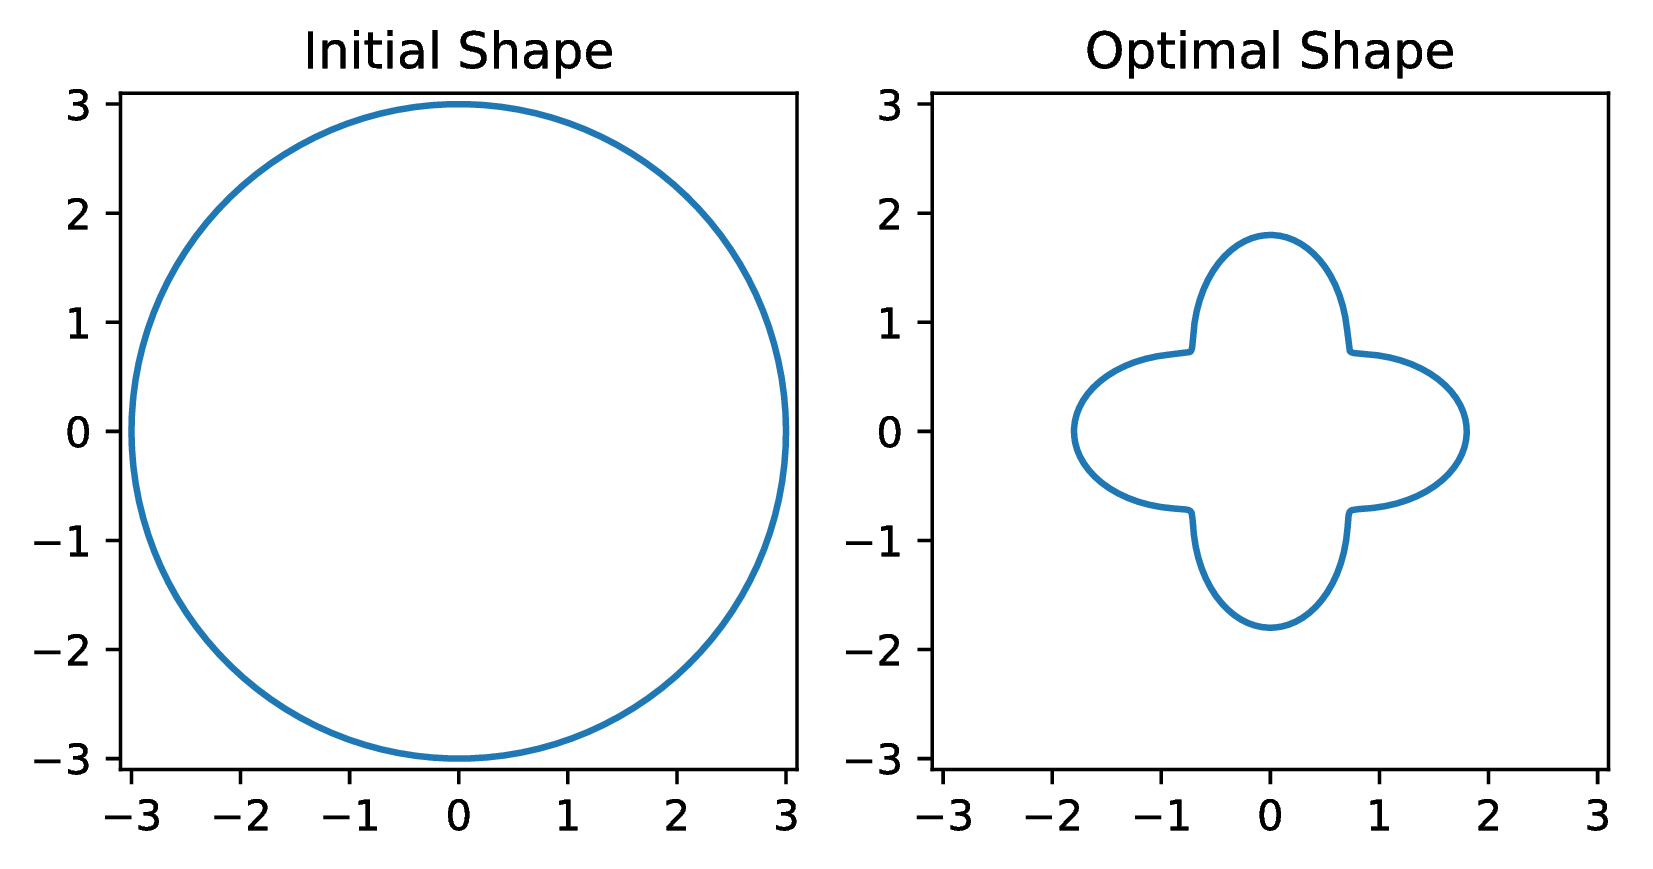
\includegraphics[width=0.7\textwidth]{./img/levelset/levelset_init_optim.png}
    \end{center}
\end{frame}
\begin{frame}{The mesh degenerates and the optimization fails}
    \begin{center}
        \includemovie[width=0.68\linewidth]{./img/levelset/levelset_grad}
    \end{center}
\end{frame}
\begin{frame}[c]
    \begin{center}
        \vspace{0.6cm}
        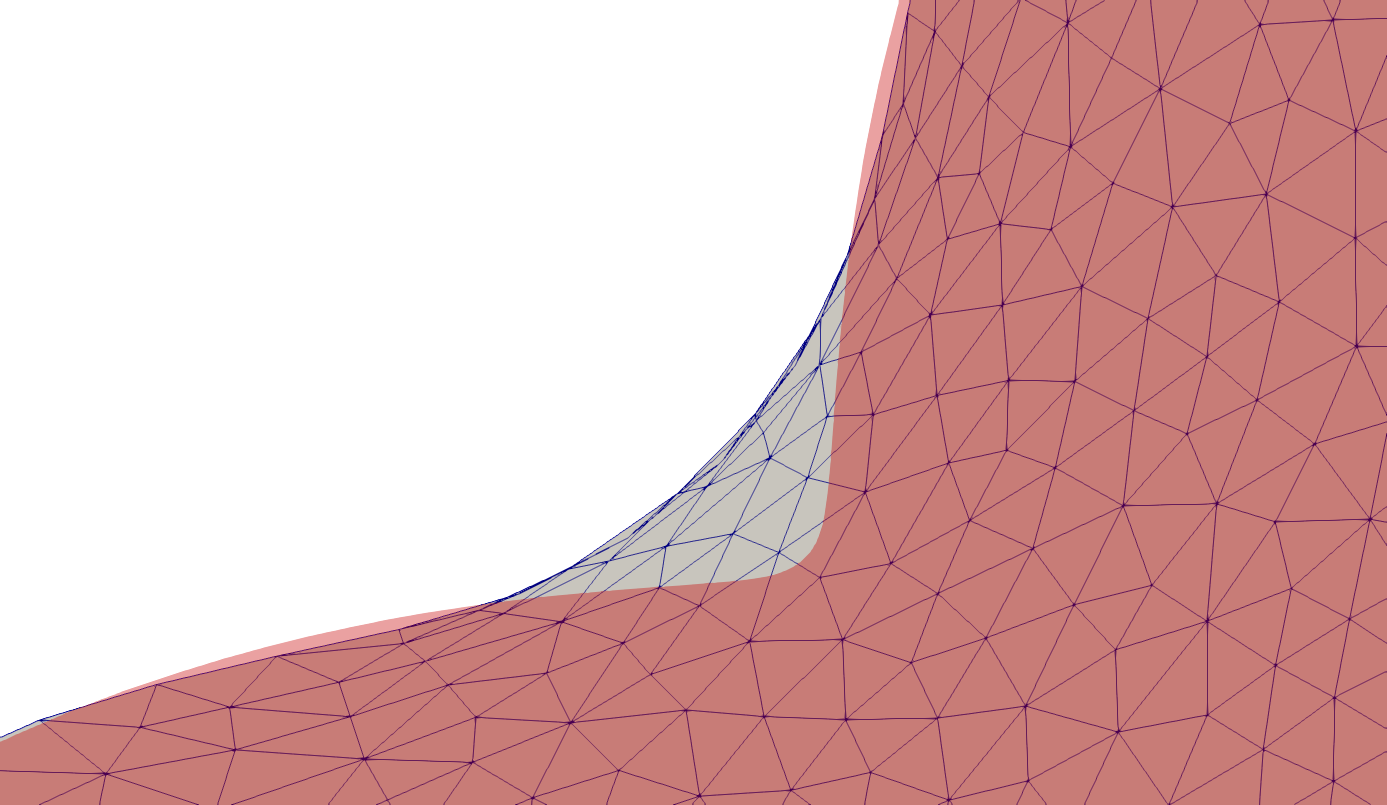
\includegraphics[width=\linewidth]{./img/levelset/levelset_grad_final.png}
    \end{center}
\end{frame}
\begin{frame}{Riemannian Mapping Theorem}
    \begin{definition}[Conformal Mapping]
        Let $\Omega\subset\re^2$. A vector-field $\ub=(u,v):\Omega\to \re^2$ is called \emph{conformal} if it satisfies the \emph{Cauchy-Riemann equations}
        \begin{equation}
            \Bc\ub \defeq \begin{pmatrix}
                \partial_x u - \partial_y v\\
                \partial_y u + \partial_x v 
            \end{pmatrix} = 0.
        \end{equation}
        Conformal mappings are \emph{angle preserving}.
    \end{definition}
    \begin{theorem}[Riemannian Mapping Theorem]
        Let $\Omega,\ \Omega' \subset\re^2$ be two simply connected domains, then there exists a conformal mapping $\ub:\Omega\to \Omega'$.
    \end{theorem}
    \begin{ideablock}{Idea}
        Can we use conformal mappings in shape optimization?
    \end{ideablock}
\end{frame}
\begin{frame}
    \only<1>{
        \begin{equation}
            \begin{aligned}
                & \underset{\Omega}{\text{minimize}}
                & & J(\Omega, u)\\
                &\text{ subject to } && \Omega \in K\\
                &&& e_{\Omega}(u) = 0
            \end{aligned}
        \end{equation}
    }
    \only<2->{
        \begin{equation}
            \begin{aligned}
                & \underset{\Omega}{\text{minimize}}
                & & J(\Omega)
            \end{aligned}
        \end{equation}
    }
    \only<3->{
        \begin{itemize}
            \item Let $H$ be a Hilbert space of vector-fields defined on $\Omega$ (think $H=H^1(\Omega;\re^2)$).
            \item The shape derivative is then given by 
                \begin{equation}
                    \Dr J(\Omega)[\vb] = \lim_{h\downarrow 0} \frac{J((\idb+h\vb)(\Omega)) - J(\Omega)}{h}
                \end{equation}
            \item Hadamard Theorem: there exists a $g:\partial\Omega\to\re$ such that 
                \begin{equation}
                    \Dr J(\Omega)[\vb] = \int_{\partial\Omega} g \vb\cdot \nb \dr \xb \quad \text{ for all } \vb\in H.
                \end{equation}
        \end{itemize}
    }
\end{frame}
\begin{frame}{From derivative to gradient}
    \begin{itemize}
        \item The gradient at $\Omega$ is defined as the element $\ub\in H$ such that 
            \begin{equation}
                (\ub, \vb)_H = \Dr J(\Omega)[\vb].
            \end{equation}
        \item One can show that $\frac{-\ub}{\norm{\ub}_H}$ solves 
            \begin{equation}
                \min_{\vb\in H: \norm{\vb}_H=1} \Dr J(\Omega)[\vb].
            \end{equation}
    \end{itemize}
\end{frame}
\begin{frame}
    \begin{example}
        If we pick $H=[\mathring{H}^1(\Omega)]^2$ and 
            \begin{equation}
                (\ub, \vb)_{\mathring{H}^1} \defeq \int_{\Omega} \nabla \ub\colon \nabla \vb \dr \xb
            \end{equation}
            then the equation for the shape gradient becomes
            \begin{equation}
                \int_{\Omega} \nabla \ub\colon \nabla \vb \dr \xb = \int_{\partial\Omega} g\vb\cdot\nb\dr\xb
            \end{equation}
            This is the weak form of 
            \begin{equation}
                \begin{aligned}
                    - \Delta \ub &= 0 && \text{ in }\Omega,\\
                    \frac{\partial\ub}{\partial\nb} &= g\nb && \text{ on }\Omega.
                \end{aligned}
            \end{equation}
    \end{example}
\end{frame}
\begin{frame}
    \begin{example}
        If we pick $H=\mathring{H}^1(\sym; \Omega)$ and 
            \begin{equation}
                (\ub, \vb)_{\mathring{H}^1(\sym)} \defeq \int_{\Omega} \sym(\nabla \ub)\colon \sym(\nabla \vb) \dr \xb
            \end{equation}
            then the equation for the shape gradient becomes
            \begin{equation}
                \int_{\Omega} \sym(\nabla \ub)\colon \sym(\nabla \vb) \dr \xb = \int_{\partial\Omega} g\vb\cdot\nb\dr\xb
            \end{equation}
            This is the weak form of 
            \begin{equation}
                \begin{aligned}
                    - \div(\sym(\nabla \ub)) &= 0 && \text{ in }\Omega,\\
                    \sym(\nabla \ub) \nb &= g\nb && \text{ on }\Omega.
                \end{aligned}
            \end{equation}
    \end{example}
\end{frame}

\begin{frame}
    \begin{itemize}
        \item Alternative view-point: shape gradient $\ub$ solves
            \begin{equation}
                \min_{\vb\in H} \frac{1}{2}\norm{\vb}_H^2 - \Dr J(\Omega)[\vb].
            \end{equation}
        \item We want to restrict ourselves to deformations that are conformal:
            \begin{equation}
                \min_{\vb\in H:\textcolor{red}{\Bc \vb = 0}} \frac{1}{2}\norm{\vb}_H^2 - \Dr J(\Omega)[\vb].
            \end{equation}
        \item This problem does not always have a non-trivial solution, so consider instead
            \begin{equation}
                \min_{\vb\in H} \frac{1}{2}\left[\norm{\vb}_H^2 + \textcolor{red}{\frac{1}{\alpha} \norm{\Bc\vb}_{L^2}^2}\right] - \Dr J(\Omega)[\vb], \quad \text{ for } \alpha>0.
            \end{equation}
    \end{itemize}
\end{frame}
\begin{frame}
    \begin{itemize}
        \item This is simply the gradient with respect to the new inner-product
            \begin{equation}
                (\ub, \vb)_{H+\CR(\alpha)} \defeq (\ub, \vb)_H + \frac{1}{\alpha} (\Bc\ub, \Bc\vb)_{L^2}
            \end{equation}
    \end{itemize}
    \begin{ideablock}{Intuition}
        The new inner-product changes the geometry of the function space $H$ so that non-conformal functions are penalized.
    \end{ideablock}
\end{frame}
\begin{frame}
    \begin{theorem}[Decomposition]
        Bla bla bla
    \end{theorem}
    \begin{ideablock}{Intuition}
        \begin{itemize}
            \item We can decompose the gradient into a conformal and a non-conformal part.
            \item As $\alpha\to0$, the non-conformal part vanishes.
        \end{itemize}
    \end{ideablock}
\end{frame}
\begin{frame}{Numerical example}
    \begin{adjustwidth}{-3em}{-3em}
        \begin{center}
            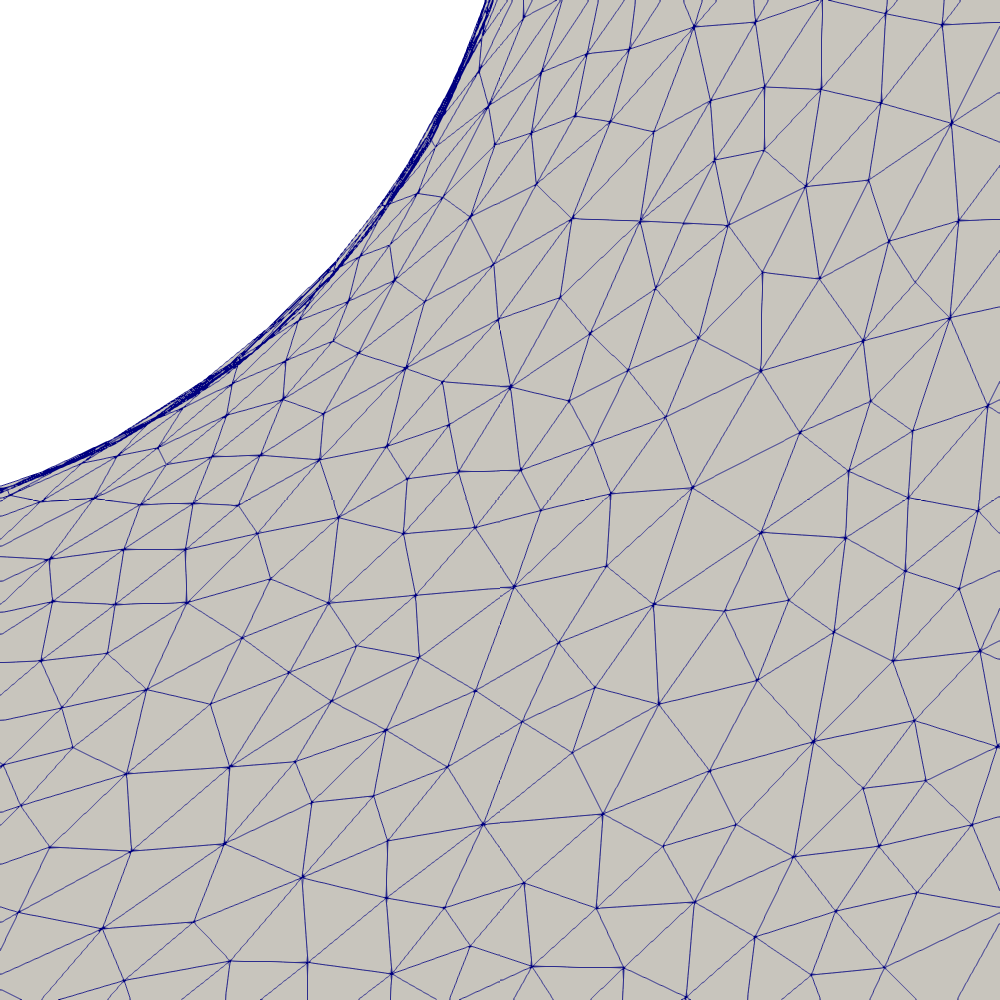
\includegraphics[width=0.37\textwidth]{./img/levelset/grad_mesh_zoom.png}
            \hspace{0.1cm}
            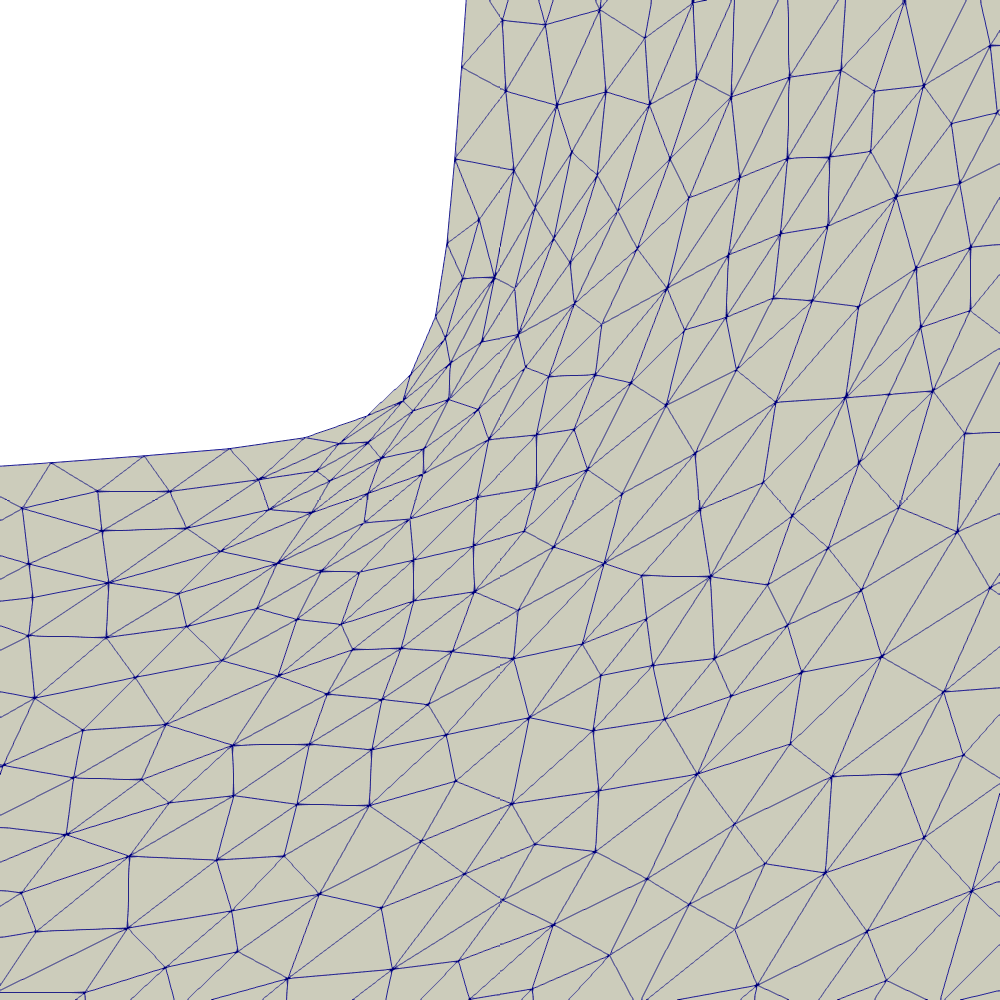
\includegraphics[width=0.37\textwidth]{./img/levelset/sym_grad_mesh_zoom.png}
            \hspace{0.1cm}
            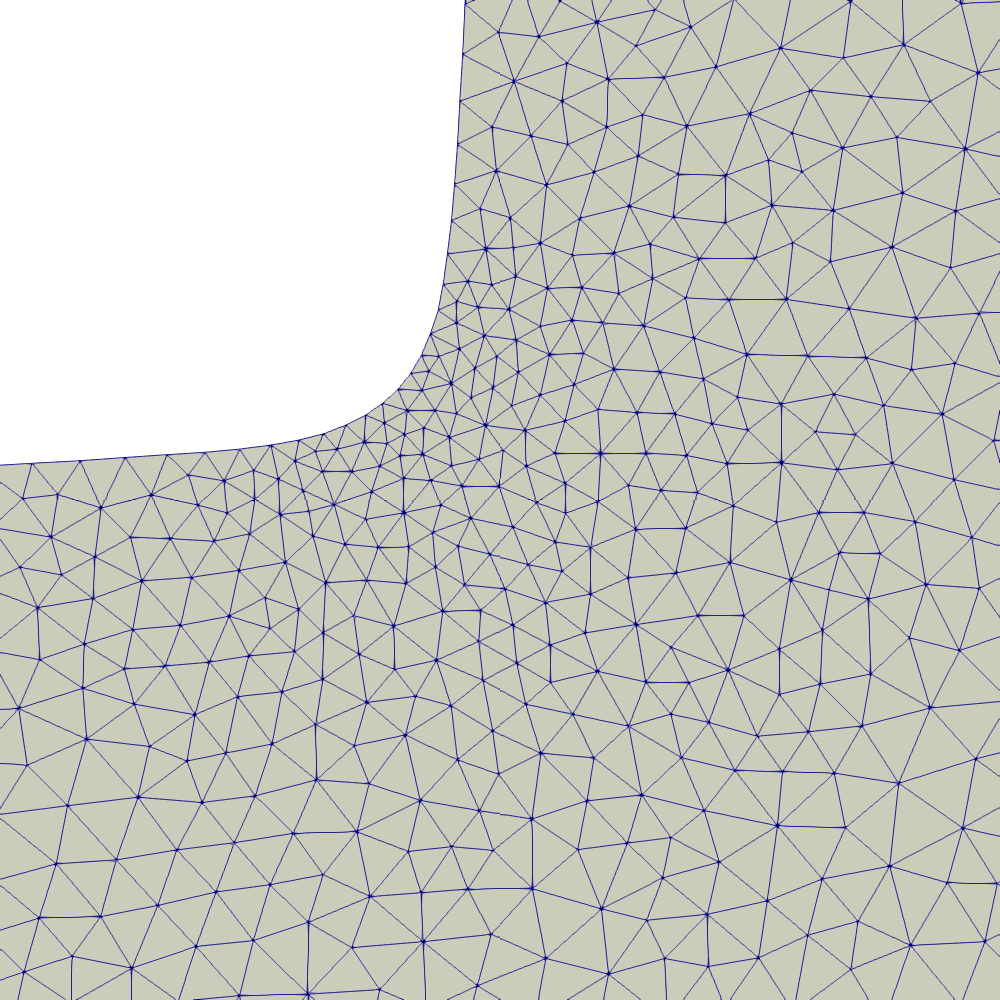
\includegraphics[width=0.37\textwidth]{./img/levelset/CR_sym_grad_1e-2_mesh_zoom.png}\\
        \end{center}
    \end{adjustwidth}
    \begin{center}
        Optimal shapes obtained when using previous inner-products (left and center) vs when using the augmented inner-product (right).
    \end{center}
\end{frame}
\end{document}






